\documentclass{article}
\usepackage[utf8]{inputenc}


\title{Challenge Computer Vision for Remote Sensing  TUB -- WS23}
\author{Matthias Jean Théo Personnaz (Matrikelnummer 486656)}
\date{\nodate}
\newcommand\scalemath[2]{\scalebox{#1}{\mbox{\ensuremath{\displaystyle #2}}}}
\usepackage{amssymb}% http://ctan.org/pkg/amssymb
\usepackage{pifont}% http://ctan.org/pkg/pifont
\newcommand{\cmark}{\ding{51}}%
\newcommand{\xmark}{\ding{55}}%
\newcommand{\vect}[1]{\mathbf{#1}}
%\documentclass[a4paper, 11pt]{report}
%\documentclass{article}  https://www.overleaf.com/project/646f741e771f71b39f00e15f
\usepackage[left=1cm, right=1cm, top=.3cm, bottom=1.6cm]{geometry}

% language related packages
\usepackage[english]{babel}
\usepackage{amsmath}
\usepackage{pdfpages}
\usepackage{geometry}
\usepackage{mathtools}
\usepackage{unicode-math}
\usepackage{stmaryrd}
\usepackage{dsfont}
% math related packages
   % add e.g equation-environment for offset equations
\usepackage{amssymb}    % add some math symbols
%\usepackage{amsthm}     % add theorem environments
\usepackage{polynom}
\usepackage{ntheorem}	% for nicer theorem environments
\usepackage{esvect}
\usepackage{todonotes}      % add todonotes
\usepackage[thinc]{esdiff}
\usepackage{listings}
\usepackage{color}
\usepackage{color,soul}
\usepackage{bbm}
\definecolor{dkgreen}{rgb}{0,0.6,0}
\definecolor{gray}{rgb}{0.5,0.5,0.5}
\definecolor{mauve}{rgb}{0.58,0,0.82}
\usepackage{tabularx}
\lstset{frame=tb,
  language=Python,
  aboveskip=3mm,
  belowskip=3mm,
  showstringspaces=false,
  columns=flexible,
  basicstyle={\small\ttfamily},
  numbers=none,
  numberstyle=\tiny\color{gray},
  keywordstyle=\color{blue},
  commentstyle=\color{dkgreen},
  stringstyle=\color{mauve},
  breaklines=true,
  breakatwhitespace=true,
  tabsize=3
}

\usepackage{hyperref}


\usepackage[toc,page]{appendix}
% layout related packages
\usepackage{titlesec}
\usepackage{parskip}		% no intendations
\usepackage{fancyhdr}       % for modifications of e.g. page layout
\usepackage{enumitem}       % for customizing itemize and enumerate labels
\usepackage{chngcntr}		% changing counters
\usepackage{amsmath}
\usepackage{mathtools}
\usepackage{pdflscape}      % landscape for fixing long polydiv
% graphic related packages
\usepackage{aligned-overset}            % align overset
\usepackage[svgnames,dvipsnames]{xcolor}	
%\usepackage{color, colortbl}


\definecolor{Gray}{gray}{0.85}

\usepackage[makeroom]{cancel}
\usepackage[normalem]{ulem}
\usepackage[makeroom]{cancel}
\usepackage{mathtools}
% referencing objects
\usepackage{cleveref}
\usepackage{bbold}
\usepackage{MnSymbol}


\NewDocumentCommand{\codeword}{v}{\texttt{#1}}


\newcommand{\codewordred}[1]{\texttt{\textcolor{red}{#1}}}
\newcommand{\codewordblue}[1]{\texttt{\textcolor{blue}{#1}}}
\newcommand{\codewordgreen}[1]{\texttt{\textcolor{black}{#1}}}


% change chapter shape
\titleformat{\chapter}[frame]{\bfseries}{\enskip \Large Lecture \;\thechapter \enskip}{8pt}{\vspace{10pt} \LARGE \centering\MakeUppercase}%
\titlespacing{\chapter}{0pt}{0pt}{10pt}

\polyset{%
   style=C,
   delims={\big(}{\big)},
   div=:
}


 
\usepackage[T1]{fontenc}
\usepackage{inconsolata}

\usepackage{color}

\definecolor{pblue}{rgb}{0.13,0.13,1}
\definecolor{pgreen}{rgb}{0,0.5,0}
\definecolor{pred}{rgb}{0.9,0,0}
\definecolor{pgrey}{rgb}{0.46,0.45,0.48}

\begin{document}

\maketitle
\vspace{-0.5cm}
\textbf{Note: All codes and figure sources not handed out are on my  \href{https://github.com/MatthiasPersonnaz/cv4rs-code-challenge}{GitHub}. Precise  parameters are only provided in this report  for the  one handed-out model (\S \ref{classical_resnet}).}
\section{Overall technical choices}

\paragraph{Dataset-driven}
%The data set is comprised of 10 classes of satellite imagery whose overall aspects are quite level. Land pictures taken from above on that small images are quite uniform and are very restricted in color shades with mostly darkish average, situated mainly on the greens and blues on the color palette. That is: similar to how medical image processing has little to do with general-purpose world images AIs, here, using a resnet as provided in the example would probably be superfluous. Because all images are the same size, with poor resolution, and taken from the same distance, all features are potentially human structures of same order of magnitude scale, so any  U-net approach,  to bypass higher orders of magnitudes in pattern sizes, is of no use for such small images.

The dataset consists of 10 classes of satellite imagery that exhibit a uniform overall appearance. These aerial images primarily capture land features and are characterized by limited color variation, predominantly in darker tones, primarily falling within the green and blue regions of the color spectrum. In a way analogous to how medical image processing differs significantly from general-purpose image recognition AI, utilizing a ResNet model, as demonstrated in the example, might be unnecessary in this context. Given that all images share the same dimensions, possess low resolution, and are taken from a consistent distance, any attempt to apply a U-Net approach, aimed at accommodating vastly different pattern scales, would be impractical for these relatively small, homogenous images.

\paragraph{Python environment-driven} Likewise, the provided \codeword{.yaml} environment does contain only general packages, for example, no \codewordblue{sklearn} for easier implementation of cross-validation, etc. With only the pretrained \codewordgreen{torchvision} models at ouor disposal, that limited the possibilities of reusing already ridiculously large models anyway (for example, \codewordgreen{torchvision.models.efficientnet\_b0} following \cite{Tan2019-az} starts at 5M+ parameters). Likewise, most of HuggingFace pretrained models are very big.


Because of these constraints and the arguably intuitive hypothesis that the complexity of the data set is very low (the meaning of complexity here is to be precised, but it could refer to the entropy of the latent space of these 10 classes), I therefore chose to build simple tailored networks in a regular train/validation-divided data set framework. Moreover, I only had access to a somewhat slow GTX~1650 mobile\footnote{About 10 times less theoretical FP32 TFLOPS than an A100, but the VRAM makes it more crippled anyway.}  with limited usable VRAM $<$4GB, filling quite fast during training and rapidly hitting the OOM killer \codewordred{RunTimeError: CUDA out of memory}   for networks reaching $\approx 10^6$ trainable parameters even for relatively small  batches, because of torch's implementation overhead and additional information required to store the batches and the models.

Because of that, I've stuck to simpler, purpose-tailored models not exceeding the  order of magnitude of a few $10^5$  parameters in size. 


\section{Overview of tested approaches}
In a few days, I tested mainly 3 (families of) approaches: 
\begin{itemize}
    \item A SimCLR  contrastive learning framework following the work of \cite{Chen2020-uz};
    \item A non-sequential model leveraging the 2D Fourier spectrum or Sobel filtering of each image;
    \item A sequential convolution  model with its variants (hyperparameters, pooling, normalization, etc) and a  non-sequential convolution model with partial or total residual connections following the work of \cite{He2015-bw}.
\end{itemize}


Every network stacks convolutions with the classical  \cite{Ronneberger2015-ib} approach ordering Conv2d $\rightarrow$ BN $\rightarrow$ ReLU ($\rightarrow$ MaxPool). Layers ranged from 4 to 8 with 16 to 64 convolution filters each, of size 6 to 15. Padding was introduced to allow for skip connections when necessary or to avoid resolution shrinking. A 80/20 train/validation random split was performed for each model of neural networks except SimCLR. No test subset was drawn, in order not to deplete the dataset too much, which was not huge (overall about 11,000 images). The dataset class remained that defined by the guidelines except for SimCLR, for which the dataset  was subsequently mutated into a new dataset of tuples of augmented images.

\subsection{[discarded] SimCLR framework to learn distambiguishing the classes from scratch to extract relevant features}
The task of classifying images for few classes suggests that SimCLR is the perfect way to go.
So I implemented it. Augmentation was performed only through rotations and color jittering / contrast / luminosity.

Since all images are from satellite imagery, with same scale in the dataset, trained to discriminate (simple multiclass classification) nor upscaling was used.

Recall SimCLR tries to minimize the following loss function for a batch $B$ of $N$ pairs of augmented images:

\begin{equation}
    \mathcal{L} =- \frac{1}{N} \sum_{i,j\in B}\log \frac{\exp(\text{sim}(z_i,z_j)/\tau)}{\sum_{k=1}^{2N}\mathbb{1}_{[k\neq i]}\exp(\text{sim}(z_i,z_k)/\tau)}
    % =-\text{sim}(z_i,z_j)/\tau+\log\left[\sum_{k=1}^{2N}\mathbb{1}_{[k\neq i]}\exp(\text{sim}(z_i,z_k)/\tau)\right]
\end{equation}



After tinkering with the temperature and SGD learning rate hyperparameters, a point of fast and efficient convergence was reached (figure \ref{fig:simclr_loss}). Unfortunately, a t-SNE embedding of the encoder's latent representations shows that the separation is very poor except for a few couple of classes (figure \ref{fig:tsne}). Later, a simple MLP classifier failed to converge sactisfactorily.




\subsection{[discarded] Bifold neural network with Fourier resp. Sobel transform}
\label{fourier_model}
\paragraph{Fourier transformation  leveraging} The intuition came from my knowledge of classical computer vision satellite images feature many regularities, typical frequencies, whether it's buildings or crops, quite universal in their appearance. Consequently, one can extract the energy spectrum of the images for leveraging regularities in those frequencies to help tell the classes apart. In figure \ref{fig:sobel_fourier}, it stands obvious that those structures exist. The spectrum of water bodies has a characteristic noise to it, unlike crops that have strong harmonics often organized in a wind rose.

So I created multpiles variations of a network (figure \ref{fig:freqcnn}) performing recognition from both the image and its Fourier \emph{square root power spectrum} (i.e. $|\mathcal{F}(\vect{x})(\vect{k})|  \sqrt{\vect{k} \cdot \vect{k}} \, \, \mathrm{d} \vect{k}$ like the signal processing equivalent) on its own small convnet in parallel with the image, and then linearly combining the  features of both the  to predict the class.


During my experiments, I found that \textbf{a relatively small 93~000 parameter network (including Fourier pattern recognition) could achieve the same  validation accuracy as a $5 \times$ to $7\times$ bigger residual convolutional network (of same depth but different resolution) without Fourier analysis}. This corroborates that the the spectrum  carries useful information indeed in the context of satellite imagery.

\paragraph{Sobel transformation leveraging} 
The same was done with the Sobel transform (which is equivalent to imposing  a very small linear convolution at the very beginning of the network), although it does not seem that this technique improved the results any more. 


\subsection{[chosen] Traditional convolution ResNet}
\label{classical_resnet}
Getting back to simplicity, the final chosen model consists of a  semi-sequential ResNet of only $\sim 213 \times 10^3$ parameters, totalling 6 layers of decreasing resolution from 64 to 16, alternating skip  residual connections and simple max pooling. Its small size compared to other models I have trained overall makes it by far the \textbf{most efficient network found}, and thus, the chosen one to hand out. The number of layers and resolution (number of convolution filters) were set given the following: 
\begin{itemize}
    \item While the dataset features a relatively diverse extent of ``canonical features'', representing shades, patterns, edges, shapes;
    \item Only a few of them should suffice to identify the class \emph{without much subsequent abstract post-processing}.
\end{itemize}
Therefore, not much abstraction is needed, cf. the first section of this report. Thus we do not need to overengineer the network by setting an outstanding depth, which only helps in case of extremely varied datasets featuring high-level features objects in size, lighting, 3D view, etc. But we still need \emph{an uncompressible number of pattern filters} to have a sufficient grasp of the scenery, thus beginning by extracting 64 of them. 
One final linear layer classifies with the visual features. It achieves a 90\% validation accuracy after less than 80 epochs of medium batches of size 50 (figure \ref{fig:loss_acc_conv}). The algorithm used was the \texttt{torch.optim.SGD} implementation of SGD with the default parameters: learning rate $lr=10^{-3}$ and momentum $\mu=0.9$. A dropout rate of 5\% for the visual features was added during training before the linear layer. The chosen loss for such classification tasks has obviously been the cross-entropy for the logits.

\paragraph{Room for improvement} To help nonlinear behaviours to emerge, adding one or more layers might help, as well as maybe th nnumber of filters to generalize more over the set of geographical configurations. In later revisions of the network, I would increasing the dropout rate and tweaking the SGD parameters for this task. I remain convinced that a SimCLR-like framework might very helpful to discriminate the classes, even though it is trickier and I was not able to find the proper hyperparameters. I think it might benefit from a larger dataset of images with finer resolution. 

\begin{figure}[h]
    \centering
    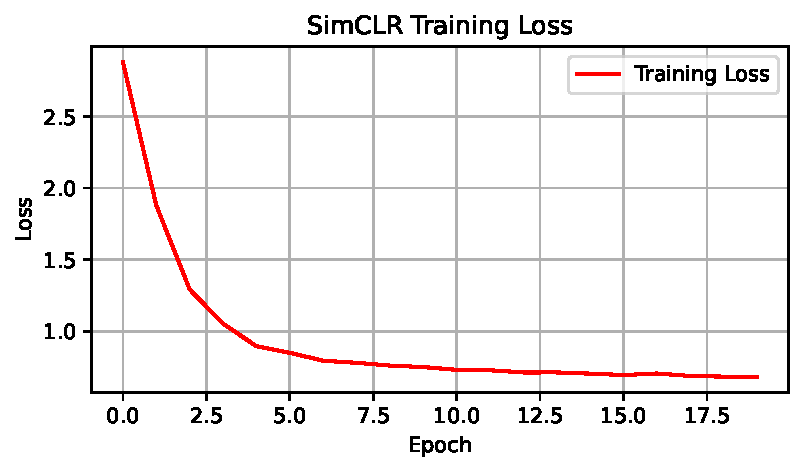
\includegraphics[scale=.6]{losses_simclr.pdf}
    \caption{SimCLR loss (including encoder and projector head). The SGD algorithm converged well.}
    \label{fig:simclr_loss}
\end{figure}

\begin{figure}[h]
    \centering
    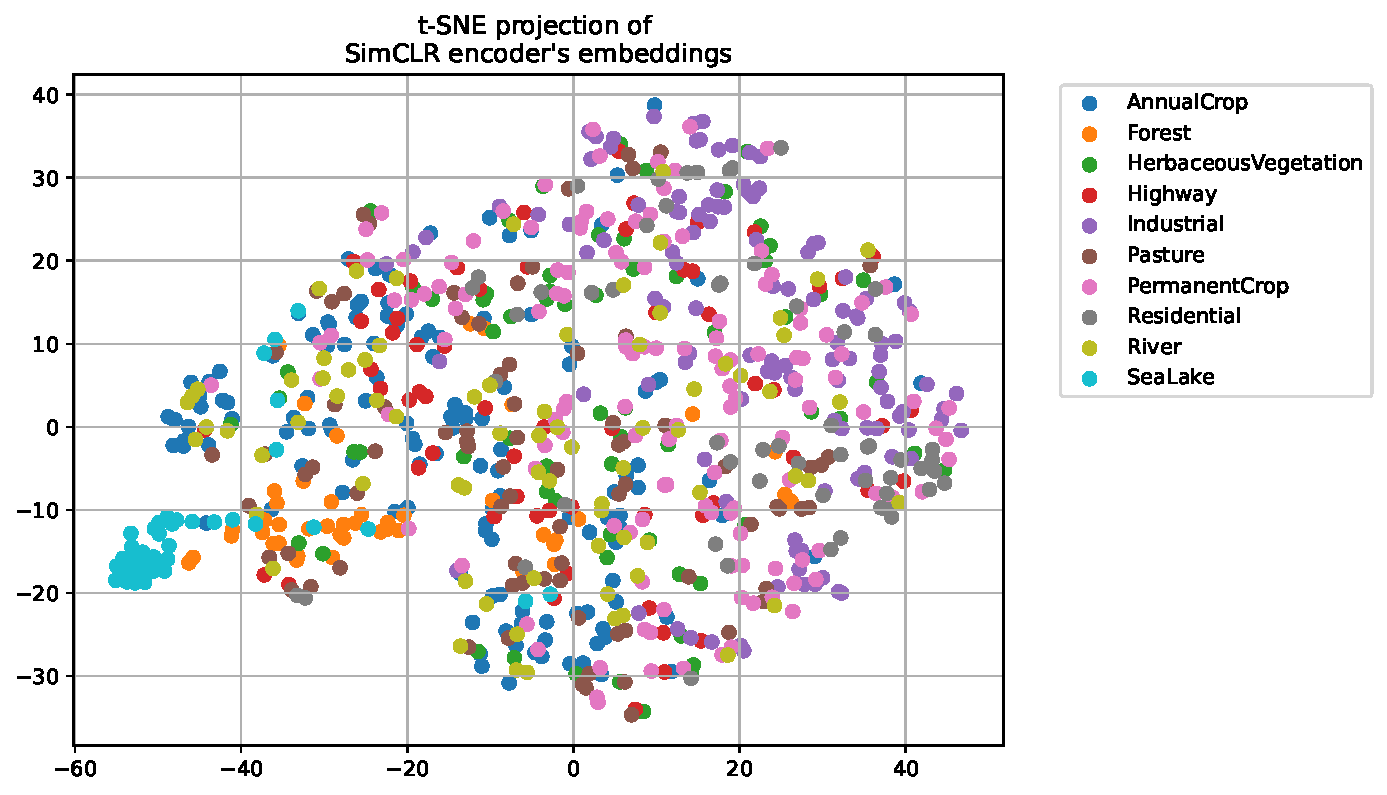
\includegraphics[scale=.6]{tsne.pdf}
    \caption{t-SNE projection of SimCLR's encoder in 32 dimensions. Although the embedding can definitely tell apart some categories (for exemple, Forest and Industrial do not overlap), the separation of the classes is still unusable to feed in a downstream classifier.}
    \label{fig:tsne}
\end{figure}


\begin{figure}[h]
    \centering
    \includegraphics[scale=.39]{viz_fourier.png}
    \caption{Original, B\&W, half-subsampled Fourier logarithmic power spectrum and Sobel filters respectively applied to a few examples drawn from the dataset. Clearly, the Fourier transform does provide some insight about the landscape although it cannot discriminate every pair of classes entirely.}
    \label{fig:sobel_fourier}
\end{figure}

\begin{figure}[h]
    \centering
    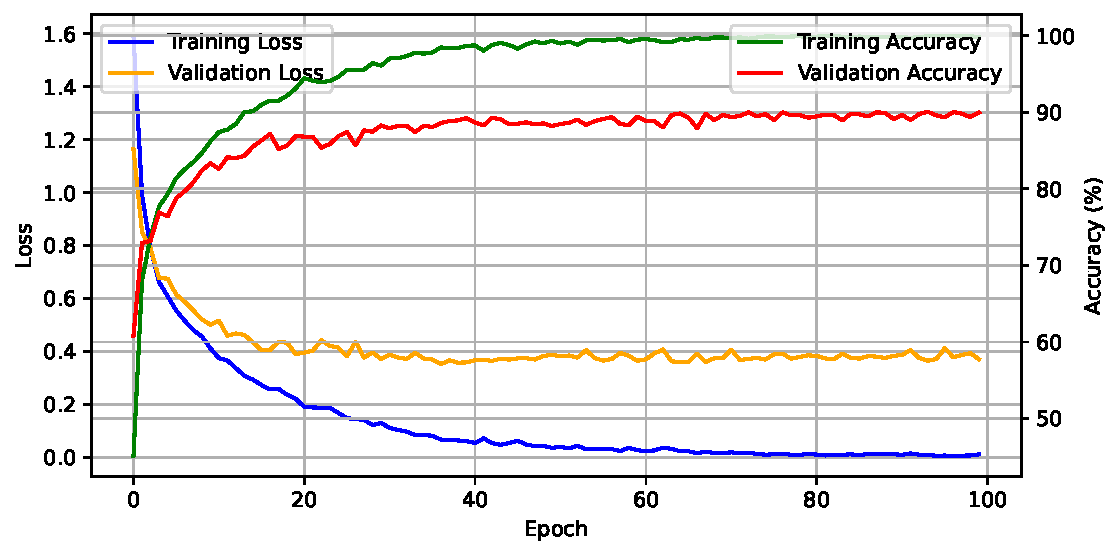
\includegraphics[scale=.8]{loss_accuracy_v5.pdf}
    \caption{Accuracy and loss of the small semi-sequential ResNet. Convergence is fast and shows the simpler models are sometimes the best for simple tasks.}
    \label{fig:loss_acc_conv}
\end{figure}

\begin{figure}[h]
    \centering
    \includegraphics[scale=.3]{graph_freqcnn.pdf}
    \caption{Graph of the non-sequential, partially residual model leveraging the Fourier transform (model in \S \ref{fourier_model}). The specific number of parameters and layers is  irrelevant on the figure and bigger configurations were tested for that architecture. The other architectures tested for the Sobel transform and semi-sequential simple ResNets were either very similar, or only included the right branch of this network respectively. Thus they are not shown in this report to avoid redundancy.}
    \label{fig:freqcnn}
\end{figure}

\newpage
\nocite{*}
\bibliographystyle{alpha} %abbrv % alpha % unsrt
\bibliography{biblio.bib} 


\end{document}



\begin{appendices}
    \section{Section 1}
\end{appendices}